\documentclass[10 pt,spanish]{article}  % Comment this line out
\usepackage[spanish]{babel}
\selectlanguage{spanish}
\usepackage[utf8]{inputenc}
\usepackage{hyperref, mathtools, listings}
\usepackage{tikz}
\usepackage{float}
\usepackage{amsmath, amsthm, amssymb, amsfonts, amscd}
\usepackage{color}
\usepackage{datetime}
%%\usepackage[table,xcdraw]{xcolor}
 
\definecolor{codegreen}{rgb}{0,0.6,0}
\definecolor{codegray}{rgb}{0.5,0.5,0.5}
\definecolor{codepurple}{rgb}{0.58,0,0.82}
\definecolor{backcolour}{rgb}{0.95,0.95,0.92}
 
\lstdefinestyle{mystyle}{
    basicstyle=\ttfamily,
    backgroundcolor=\color{backcolour},   
    commentstyle=\color{codegreen}\ttfamily,
    keywordstyle=\color{magenta}\ttfamily,
    numberstyle=\tiny\color{codegray}\ttfamily,
    stringstyle=\color{codepurple}\ttfamily,
    basicstyle=\footnotesize\ttfamily,
    breakatwhitespace=false,         
    breaklines=true,                 
    captionpos=b,                    
    keepspaces=true,                 
    numbers=left,                    
    numbersep=5pt,                  
    showspaces=false,                
    showstringspaces=false,
    showtabs=false,                  
    tabsize=2
}



\usepackage[a4paper, total={6in, 8in}]{geometry}


\lstset{style=mystyle}
\title{\LARGE \bf
Práctica de interbloqueos
}
\author{Andrea Blanco, Santiago Iglesias, Ana Martínez, \\
Manuel de Prada y Jorge Vázquez}


\begin{document}

\maketitle

\section{INTRODUCCIÓN}
Se incluye un Makefile que permite compilar todos los ejercicios. Comentamos a continuación las soluciones implementadas, atacando las condiciones necesarias para el interbloqueo.

\section{EXCLUSIÓN MUTUA}
Esta solución consiste en trasladar el trabajo que harían los hilos con los recursos a demonios. Por tanto, los hilos solo tendrían que hacer una solicitud al demonio correspondiente para que los inserte en su cola y después seguirían con su ejecución normal. Hay que asegurarse de proteger cada cola con otro mutex, sin embargo esto evita los interbloqueos con los hilos al no mantener bloqueados los recursos. 
El demonio espera hasta que la cola no esté vacía y entonces evalúa la solicitud y la elimina de la cola. Repite esto hasta que todos los hilos hayan finalizado (que controlamos en el código con una variable de condición) y se hayan procesado todas las solicitudes (la cola esté vacía).
Para intentar eliminar la desventaja de encontrarse con la cola llena, incluimos en el código lo siguiente: 
\begin{lstlisting}[language=C++,caption=Espera para inserción]
    pthread_mutex_lock(&recurso[j]); // Adquiero el recurso
    while(insertarCola(&buffer[j],thid)==-1){ //Intento insertarlo
      sleep(3); //Si no lo consigo espero y vuelvo a intentarlo
    }
    pthread_mutex_unlock( &recurso[j]);
\end{lstlisting}

De esta forma, esperará hasta que su solicitud se ponga a la cola. Debe tenerse en cuenta que hace falta compilarlo junto a la librería "cola.h"y cola.c.
\subsection{VENTAJAS}
La mayor ventaja de la solución es que evita los interbloqueos y permite que varios hilos trabajen en paralelo. También reduce el tiempo que tiene que esperar cada uno de ellos en general y permite que acaben rápidamente. Evita además carreras críticas en la cola al estar protegida con un mutex, tanto para inserción como para la evaluación y retirada del primer elemento.
\subsection{DESVENTAJAS}
Uno de los principales problemas es que no es aplicable en todos los casos. Además, nuestra solución a encontrarse con la cola llena crea una cierta desventaja en cuanto a tiempo de espera, ya que el hilo puede estar con el mutex bloqueado bastante tiempo si no consigue insertar. 
Por otro lado, no es la solución más fácil de implementar, ya que implica añadir el código de las colas con sus funciones y N hilos más. Esto conlleva un cierto retardo que en códigos con interbloqueos puntuales no sería la solución más adecuada por ser demasiado costosa.
\section{CONTENCIÓN Y ESPERA}
Para evitar la condición de contención y espera, sustituimos los lock por trylock. Cuando un hilo no consigue obtener uno de los recursos, en vez de quedarse esperando, libera todos los recursos que ya tenía y espera un tiempo aleatorio entre 0 y 5s. De esta forma, eventualmente algún proceso obtendrá todos los recursos, acabará y los otros hilos podrán progresar.
\begin{lstlisting}[language=C++,caption=Contención y espera]
    printf("Soy %d y quiero el recurso %d\n", thid, j);
    int r = pthread_mutex_trylock( & recurso[j]); // Intento adquirir el recurso
    if (r!=0){ //si no he podido conseguirlo
      printf("No he podido obtener el recurso %d\n", j);
      for (int ii = 0; ii < i; ii++) { //libero todos los recursos que tenia
        pthread_mutex_unlock( & recurso[mis_recursos[ii]]);
        printf("\tLiberado el recurso %d\n", mis_recursos[ii]);
      }
      sleep(rand()%5);// espero un tiempo aleatorio para que otros procesos acaben
      i=-1; //vuelvo con la i para que pase a 0 y vuelva empezar
      continue; //vuelvo al bucle
    }// si he conseguido el recurso, continuo normalmente
\end{lstlisting}
\subsection{VENTAJAS}
Esta solución permite que los procesos no lleguen a un interbloqueo, es rápida de implementar y no provoca comportamiento inconsistente (los programas que acaban han conseguido los recursos en exclusiva).
\subsection{DESVENTAJAS}
Los hilos pueden pasar mucho tiempo esperando, bloqueando y desbloqueando recursos, tiempo que no será productivo ni predecible. Además, en caso de que haya muchos procesos, puede ser necesario aumentar los tiempos de espera aleatoria para que la solución sea efectiva. No es una solución que escale bien en el número de recursos ni de hilos. Tampoco favorece la multitarea real.

\section{NO APROPIATIVA}
En este apartado tratamos de atacar la propiedad no apropiativa de lows interbloqueos. Para ello lanzamos un hilo, llamado hilo comprobador, que trata de buscar ciclos en el grafo que implementamos y que representa la relación entre los recursos y los hilos. Este grafo es el mismo que describe Tanenbaum, es decir, un arco de un recurso a un hilo quiere decir que el hilo posee ese recurso y, en el caso contrario, quiere decir que ese hilo desea poseer ese recurso. Así, empleamos una representación estática del grafo en una matriz cuadrada de orden el número de hilos más el número de recursos, siendo las Pmax primeras filas referentes a los hilos y las Nmax columnas restantes correspondientes a los recursos. Lo mismo para las filas.
Una vez explicada esta estructura, algoritmo es el siguiente. Cada vez que un hilo i desea obtener un recurso j accede al grafo e indica esto poniendo el la posición $(i, j + Pmax)$ un $1$. Además, eleva en uno el valor del semáforo comprobador para que el hilo que comprueba si hay ciclos se desbloquee.
\begin{lstlisting}[language=C++,caption=Acceso al grafo al desear recurso]
     //Acceso al grafo para añadir el recurso deseado
    pthread_mutex_lock(&accesoGrafo);
    printf("Soy %d y quiero el recurso %d\n", thid, j + Pmax);
    G[thid][j + Pmax] = 1; //Se añade una arista desde el hilo thid hasta el recurso j
    filaModif = thid;
    colModif = j;

    //Se permite al hilo comprobador que trabaje
    sem_post(comprobador);
    pthread_mutex_unlock(&accesoGrafo);
\end{lstlisting}
Si el hilo i consigue el recurso j, entonces vuelve a acceder al grafo y pone a cero la anterior posición y pone a uno justo la traspuesta. Así es como se va actualizando el grafo.
\begin{lstlisting}[language=C++,caption=Acceso al grafo al obtener un recurso]
     //Acceso al grafo para añadir el recurso obtenido
    pthread_mutex_lock(&accesoGrafo);
    printf(" Soy %d y tengo el recurso %d\n", thid, j + Pmax);
    G[thid][j + Pmax] = 0;
    G[j + Pmax][thid] = 1; //Se añade una arista desde el  recurso j hasta el hilo thid
    //imprimirGrafo();
    pthread_mutex_unlock(&accesoGrafo);
\end{lstlisting}
Ahora, el hilo comprobador lo que hace es esperar en el semáforo hasta que éste le permite desbloquearse, es decir, hasta que un hilo trabajador desea un recurso. En esta situación comprueba con la función hayciclo() si hay algún ciclo y, en caso de haberlo, sabe que es por culpa de la última fila modificada (filMadif) del grafo, es por eso que se la pasa a deshacerCiclo(), la cual se encarga de liberar el recurso almacenado en colModifla última columna modificada (colModif). En todo este tiempo el acceso al grafo se bloquea para que no haya interferencias con la comprobación. Este hilo sólo se lanza cuando un hilo desea un recurso y no también cuando lo obtiene porque, de forma lógica, el paso último que provoca un interbloqueo es que un hilo desee un recurso poseído por otro hilo. Lo que acabamos de decir se realiza de la siguiente forma.

\begin{lstlisting}[language=C++,caption=Hilo comprobante]
     void *hiloComprobador(void *tid){
  comprobador = sem_open("Comprobador", O_CREAT, S_IRWXU, 0);

  //Se mantiene activo hasta que acaba el hilo principal
  while(1){
    //Semáforo para controlar el trabajo (que no esté en espera activa)
    sem_wait(comprobador);
    pthread_mutex_lock(&accesoGrafo);

    //Comprueba si el grafo posee un ciclo y si lo hay lo deshace
    if(hayCiclo())
      deshacerCiclo(filaModif, colModif);
    pthread_mutex_unlock(&accesoGrafo);
  }
  pthread_exit(NULL);
}
\end{lstlisting}
Así, otros detalles del código tales como la búsqueda de ciclos y demás problemas de trabajo con grafos no serán comentados por falta de interés para esta práctica.

\subsection{VENTAJAS}
Las ventajas de esta implementación son claras, el autónomo manejo de los interbloqueos gracias a la implementación del grafo. Además, el enorme paralelismo proporcionado por el hecho de tener un hilo comprobador sin usar espera activa mejora mucho el uso de CPU.

\subsection{DESVENTAJAS}
Las desventajas son la pobre escalabilidad, pues una matriz muy grande supone un gasto considerable de memoria. Además, hay mucho uso de mutexes para acceder al grafo, por lo que los tiempos de trabajo se verán reducidos ligeramente.

\section{ESPERA CIRCULAR}

Para empezar, comentaremos brevemente en qué consiste el problema de la espera circular. Éste se basa, en el caso más sencillo, en que un proceso(A) adquiere un recurso(1), que a su vez es solicitado por otro proceso (B), que por otro lado tiene asignado otro recurso (2) que a su vez es solicitado por el proceso A; por lo que tenemos un interbloqueo. Esta situación se describe en la imagen adjunta:
\begin{figure}[H]
  \centering
  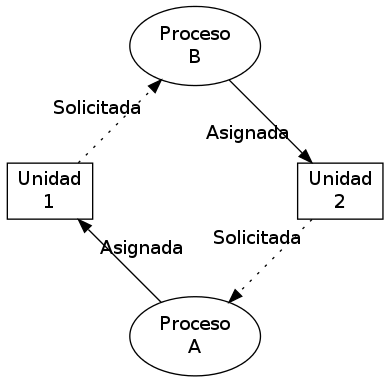
\includegraphics[scale=0.4]{bloqueo_mutuo_simple.png}
  \caption{Ejemplo del interbloqueo ocasionado por la espera circular}
  \label{fig:grafico1}
\end{figure}
Para tratar de solucionarlo, asignaremos a cada hilo un único recurso a la vez cumpliendo además que un hilo solamente puede adquirir un recurso que tenga un valor superior al que ya tenía previamente (el valor de los recursos se incrementa de forma gradual .
\begin{lstlisting}[language=C++,caption=Asignación de un recurso a un hilo en caso de sea mayor que el que ya tenía.]
     Ri = (int)(Nmax) * (rand() / (RAND_MAX + 1.0)); //Numero de recursos aleatorios <=N, siendo Nmax el numero de recursos
    int i, j;
    int mi_recurso=-1;//inicializamos el recurso a -1 para provocar que se pueda asignar el primer recurso (0) al primer hilo que entra en la funcion trabajo
    for (int i=0;i<Ri;i++){
        j=i;//Asigno el valor 
        if (mi_recurso < j) mi_recurso = j; 
  	}
\end{lstlisting}
De esta manera, es imposible que se produzca el interbloqueo, ya que en cada instante, uno de los recursos asignados será el más alto, por lo que dicho proceso nunca solicitará un recurso previamente asignado. De esta manera se presentan 2 opciones: o acaba, o solicita recursos con mayor valor que éste,los cuales estarán disponibles. En un momento dado, terminará y liberará sus recursos.y simultáneamente, algún otro proceso contendrá el recurso más alto y también podrá terminar. De esta forma, evitamos la aparición del interbloqueo al permitir la terminación de todos los hilos.
Procedemos a continuación a enumerar las ventajas e inconvenientes de dicha solución:
\subsection{VENTAJAS}
Es sencilla de implementar, permitiendo que los procesos no lleguen a un interbloqueo y permite la ejecución concurrente de varios hilos (no es necesario que un proceso coja todos los recursos y los suelte para que el resto puedan adquirirlos). 
\subsection{INCONVENIENTES}
Cada proceso debe soltar un recurso para que el siguiente lo pueda coger, por lo que los procesos permanecerán inactivos hasta el momento en el que puedan adquirir un recurso de mayor valor.  
\end{document}
